\chapter{Opis projektnog zadatka}
		
		\textbf{\textit{dio 1. revizije}}\\
		
		\textit{Na osnovi projektnog zadatka detaljno opisati korisničke zahtjeve. Što jasnije opisati cilj projektnog zadatka, razraditi problematiku zadatka, dodati nove aspekte problema i potencijalnih rješenja. Očekuje se minimalno 3, a poželjno 4-5 stranica opisa.	Teme koje treba dodatno razraditi u ovom poglavlju su:}
		\begin{packed_item}
			\item \textit{potencijalna korist ovog projekta}
			\item \textit{postojeća slična rješenja (istražiti i ukratko opisati razlike u odnosu na zadani zadatak). Dodajte slike koja predočavaju slična rješenja.}
			\item \textit{skup korisnika koji bi mogao biti zainteresiran za ostvareno rješenje.}
			\item \textit{mogućnost prilagodbe rješenja }
			\item \textit{opseg projektnog zadatka}
			\item \textit{moguće nadogradnje projektnog zadatka}
		\end{packed_item}
		
		\textit{Za pomoć pogledati reference navedene u poglavlju „Popis literature“, a po potrebi konzultirati sadržaj na internetu koji nudi dobre smjernice u tom pogledu.}
		\eject
		
		\section{Primjeri u \LaTeX u}
		
		\textit{Ovo potpoglavlje izbrisati.}\\
		%Mislim da je ovo najbolje obrisati netom prije predaje ili kad se svi
		%malo bolje upoznaju s LaTeXom, tu ima dosta korisnih primjera - Luka

		U nastavku se nalaze različiti primjeri kako koristiti osnovne funkcionalnosti \LaTeX a koje su potrebne za izradu dokumentacije. Za dodatnu pomoć obratiti se asistentu na projektu ili potražiti upute na sljedećim web sjedištima:
		\begin{itemize}
			\item Upute za izradu diplomskog rada u \LaTeX u - \url{https://www.fer.unizg.hr/_download/repository/LaTeX-upute.pdf}
			\item \LaTeX\ projekt - \url{https://www.latex-project.org/help/}
			\item StackExchange za Tex - \url{https://tex.stackexchange.com/}\\
		
		\end{itemize} 	


		
		\noindent \underbar{podcrtani tekst}, \textbf{podebljani tekst}, 	\textit{nagnuti tekst}\\
		\noindent \normalsize primjer \large primjer \Large primjer \LARGE {primjer} \huge {primjer} \Huge primjer \normalsize
				
		\begin{packed_item}
			
			\item  primjer
			\item  primjer
			\item  primjer
			\item[] \begin{packed_enum}
				\item primjer
				\item[] \begin{packed_enum}
					\item[1.a] primjer
					\item[b] primjer
				\end{packed_enum}
				\item primjer
			\end{packed_enum}
			
		\end{packed_item}
		
		\noindent primjer url-a: \url{https://www.fer.unizg.hr/predmet/proinz/projekt}
		
		\noindent posebni znakovi: \# \$ \% \& \{ \} \_ 
		$|$ $<$ $>$ 
		\^{} 
		\~{} 
		$\backslash$ 
		
		
		\begin{longtblr}[
			label=none,
			entry=none
			]{
				width = \textwidth,
				colspec={|X[8,l]|X[8, l]|X[16, l]|}, 
				rowhead = 1,
			} %definicija širine tablice, širine stupaca, poravnanje i broja redaka naslova tablice
			\hline \SetCell[c=3]{c}{\textbf{naslov unutar tablice}}	 \\ \hline[3pt]
			\SetCell{LightGreen}IDKorisnik & INT	&  	Lorem ipsum dolor sit amet, consectetur adipiscing elit, sed do eiusmod  	\\ \hline
			korisnickoIme	& VARCHAR &   	\\ \hline 
			email & VARCHAR &   \\ \hline 
			ime & VARCHAR	&  		\\ \hline 
			\SetCell{LightBlue} primjer	& VARCHAR &   	\\ \hline 
		\end{longtblr}
		

		\begin{longtblr}[
				caption = {Naslov s referencom izvan tablice},
				entry = {Short Caption},
			]{
				width = \textwidth, 
				colspec = {|X[8,l]|X[8,l]|X[16,l]|}, 
				rowhead = 1,
			}
			\hline
			\SetCell{LightGreen}IDKorisnik & INT	&  	Lorem ipsum dolor sit amet, consectetur adipiscing elit, sed do eiusmod  	\\ \hline
			korisnickoIme	& VARCHAR &   	\\ \hline 
			email & VARCHAR &   \\ \hline 
			ime & VARCHAR	&  		\\ \hline 
			\SetCell{LightBlue} primjer	& VARCHAR &   	\\ \hline 
		\end{longtblr}
	


		
		
		%unos slike
		\begin{figure}[H]
			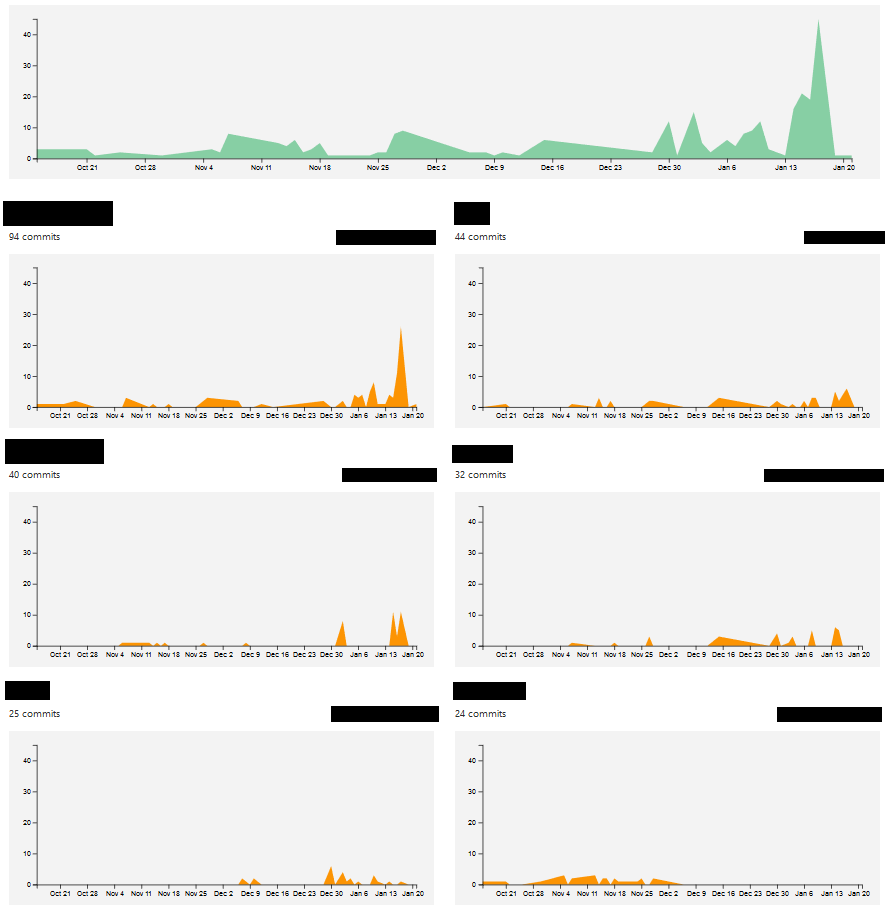
\includegraphics[scale=0.4]{slike/aktivnost.PNG} %veličina slike u odnosu na originalnu datoteku i pozicija slike
			\centering
			\caption{Primjer slike s potpisom}
			\label{fig:promjene}
		\end{figure}
		
		\begin{figure}[H]
			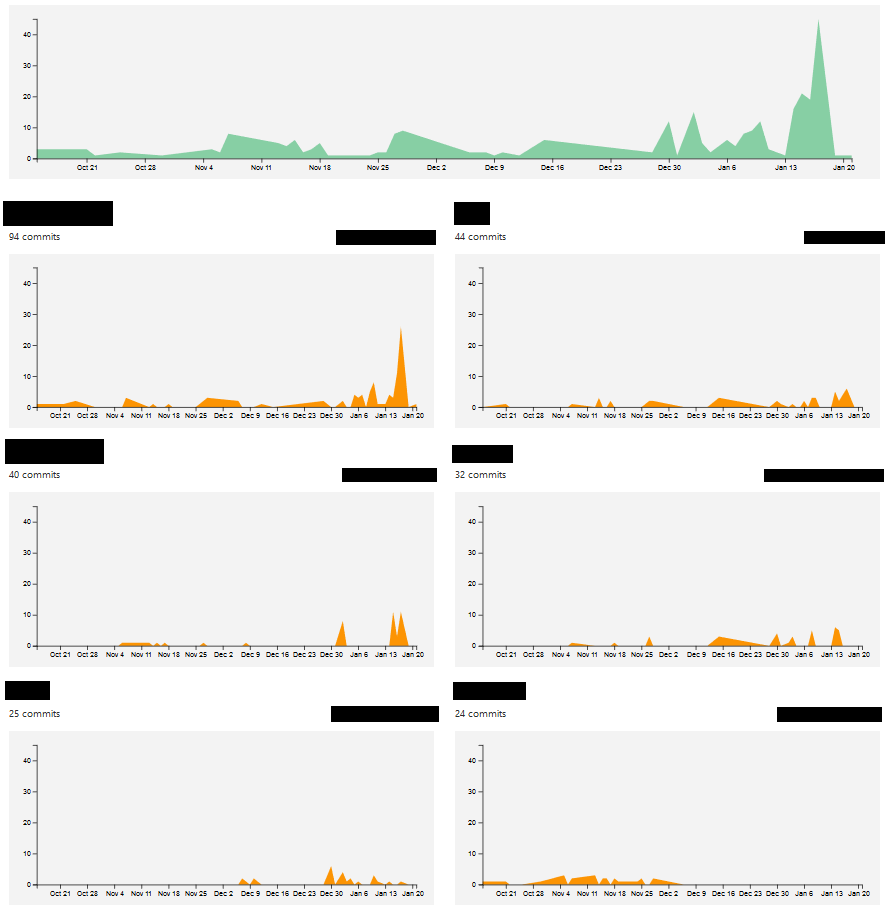
\includegraphics[width=\textwidth]{slike/aktivnost.PNG} %veličina u odnosu na širinu linije
			\caption{Primjer slike s potpisom 2}
			\label{fig:promjene2} %label mora biti drugaciji za svaku sliku
		\end{figure}
		
		Referenciranje slike \ref{fig:promjene2} u tekstu.
		
		\eject
		
		\section{Uvod}
		\raggedright Cilj ovog projekta je razvoj web aplikacije za razmjenu recepata za pripremu kolača i diskusiju između korisnika i autora recepata koja bi ljudima omogućila jednostavno isprobavanje novih jela i poboljšanje svojih kulinarskih sposobnosti.
		\section{Postojeća rješenja i njihovi problemi}
		Postoje brojna popularna slična rješenja, no uglavnom pate od loše preglednosti zbog previše prevelikih slika, puno praznog prostora i velike količine popratnog teksta koji nema veze sa sastojcima ili pripremom kao što je prikazano na slikama \ref{fig:primjer1} i \ref{fig:primjer2} u nastavku. 
		\begin{figure}[H]
			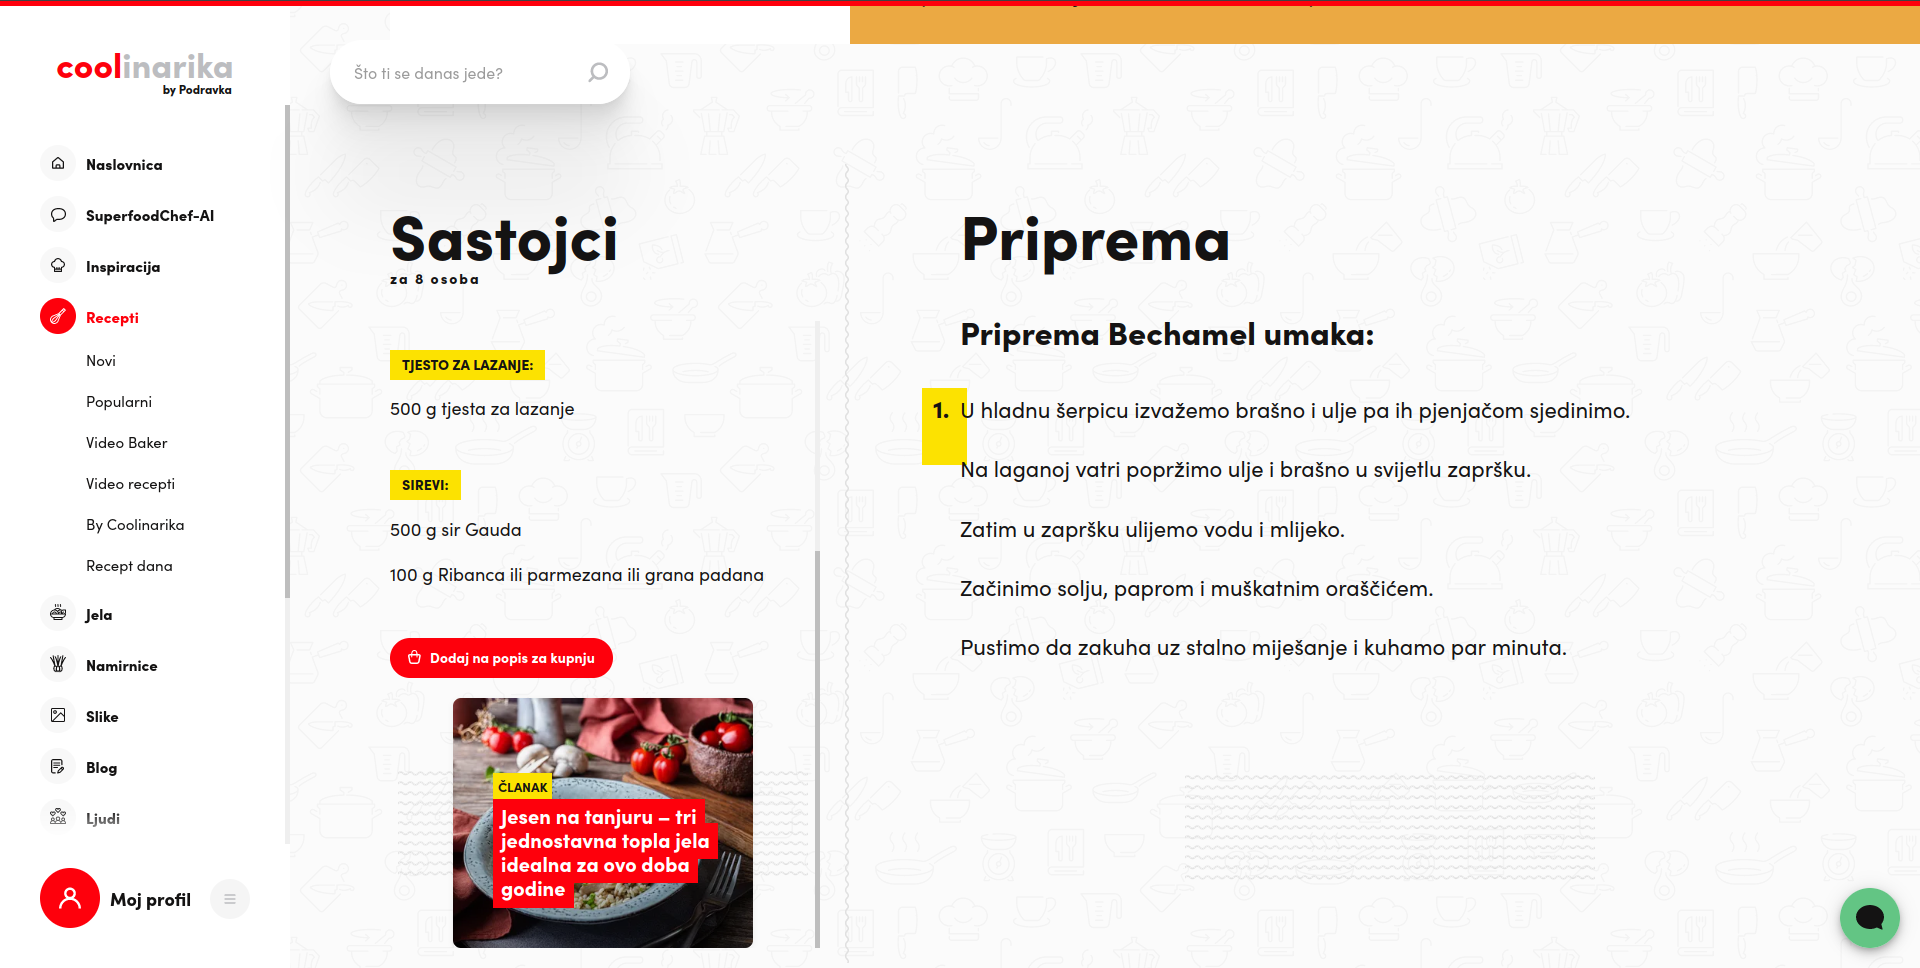
\includegraphics[scale=0.24]{slike/primjer_coolinarika.png}
			\centering
			\caption{Coolinarika - Prevelika slova, puno neiskorištenog prostora}
			\label{fig:primjer1}
		\end{figure}
		\begin{figure}[H]
			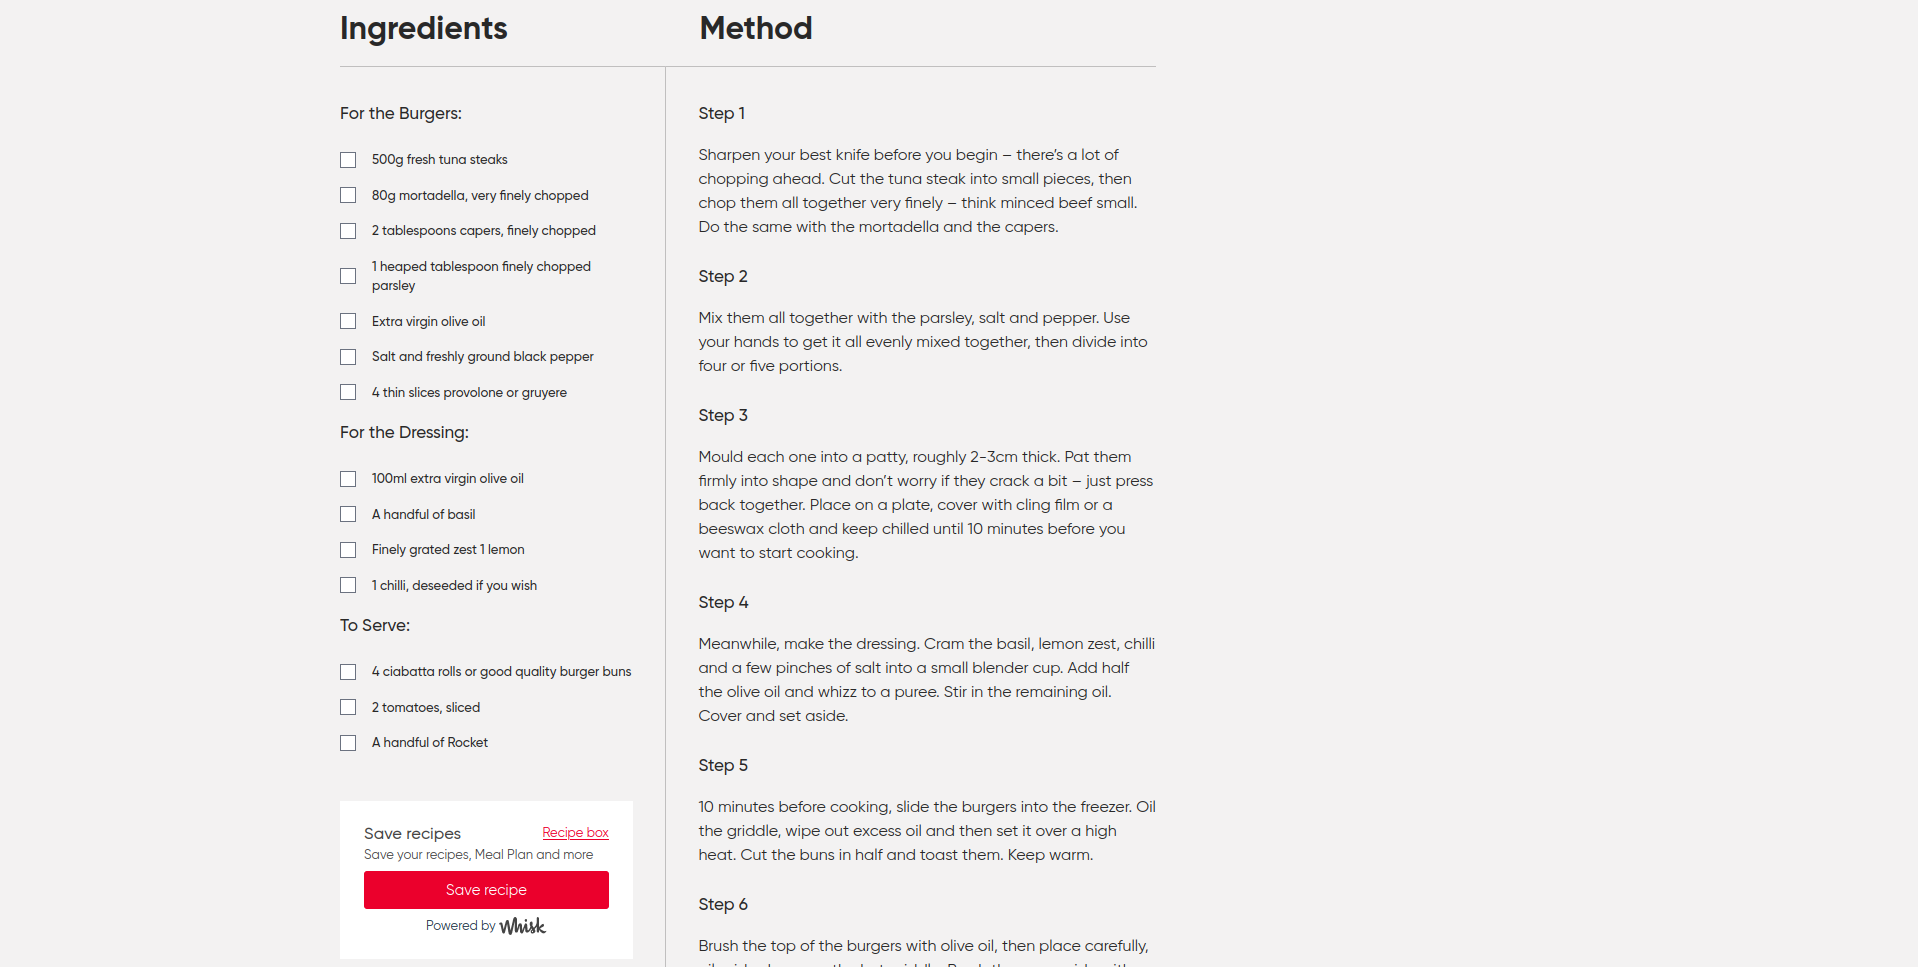
\includegraphics[scale=0.24]{slike/primjer_foodnetwork.png}
			\centering
			\caption{Foodnetwork - Preglednije, ali i dalje puno praznog prostora}
			\label{fig:primjer2}
		\end{figure}
		Recepti bi trebali sadržavati samo informacije važne za pripremu i možda jednu ili dvije uvodne rečenice. Većina recepata trebala bi stati na jednu stranicu kako bi bili pregledniji, ali i kako bi ih se lako moglo ispisati na papir. Ovakav izgled stranice nije uvijek jednostavno ostvariti, ali bi trebao uvelike poboljšati iskustvo korištenja.
		\section{Osnovne mogućnosti stranice}
		Glavna mogućnost stranice je naravno, prikazivanje sastojaka i uputa za pripremu, ali osim njih, recepti sadrže i brojne druge informacije koje olakšavaju pripremu i traženje sličnih recepata kao što su:
		\begin{packed_item}
			\item Kategorija jela
			\item Vrsta kuhinje
			\item Neuobičajeni sastojci
			\item Alergeni
			\item Vrijeme pripreme
			\item Broj porcija
			\item Ostale oznake
		\end{packed_item}
		Stranica razlikuje dvije vrste korisnika: goste, odnosno neregistrirane korisnike, i registrirane korisnike. Neregistrirani korisnici mogu pristupiti samo osnovnim funkcionalnostima stranice. Imaju potpuni pristup svim receptima te mogu pretraživati recepte po prije navedenim oznakama ili po njihovom nazivu. Isto tako mogu uz neka ograničenja pregledavati profile registriranih korisnika. Ovo će većini korisnika koji samo povremeno traže nove recepte ili inspiraciju vjerojatno biti dovoljno, a oni koji žele pristupiti naprednijim pogodnostima koje stranica nudi moraju se registrirati.
		\linebreak
		Postupak registracije vrlo je jednostavan. Potrebno je samo navesti sljedeće podatke kako bi korisnik stvorio novi profil:
		\begin{packed_item}
			\item Korisnično ime
			\item Adresu elektroničke pošte
			\item Lozinku
		\end{packed_item}
		\pagebreak
		\section{Napredne mogućnosti stranice}
		Nakon što se korisnik registrira i prijavi, otvaraju mu se brojne dodatne mogućnosti stranice. Najvažnija i najzanimljivija je naravno mogućnost objave vlastitih recepata. Kako bi korisnik objavio recept, mora navesti naziv recepta, sastojke, postupak pripreme i ukupno trajanje pripreme. Ostali podatci nisu neophodni, ali ih je korisno navesti kako bi zainteresirani korisnici mogli brže i jednostavnije naći recepte koji odgovaraju njihovim željama i potrebama.
		\linebreak
		\linebreak
		Svaki registrirani korisnik također može označavati i spremati recepte na svoj osobni profil kako bi mu u budućnosti bili lako dostupni, a isto tako mogu zapratiti druge autore kako bi bili automatski obaviješteni kada netko od njihovih najdražih autora objavi novi recept.
		Objavljeni recepti, pratitelji i osobe koje prate korisnika javno su vidljivi na profilu svakog korisnika.
		\section{Komunikacija među korisnicima}
		Osim što mogu ostavljati komentare na receptima i tako komunicirati s autorom i drugim korisnicima, registrirani korisnici također imaju mogućnost izravnog kontaktiranja autora recepata ako trebaju dodatna pojašnjenja ili žele uputiti svoje pohvale (ili kritike) autoru. Aplikacija omogućava jednostavnu razmjenu poruka između korisnika, ali isto tako, autor može navesti i druge načine na koje ga se može kontaktirati, kao što su elektronička pošta ili broj telefona. Također može navesti i vremenske periode u kojima je dostupan.
		\section{Administracija}
		Osim gostiju i registriranih korisnika, važan čimbenik u radu stranice su i administratori. Administratori imaju vlastite korisničke profile, kao i obični registrirani korisnici, ali imaju dodatne ovlasti koje im omogućavaju upravljanje stranicom.
		\linebreak
		Ovlasti administratora uključuju:
		\begin{packed_item}
			\item Upravljanje korisnicima
			\item[] \begin{packed_item}
					\item Brisanje korisnika
					\item Uređivanje korisničkih profila
					\item Dodavanje korisnika
					\end{packed_item}
			\item Upravljanje receptima
			\item[] \begin{packed_item}
					\item Brisanje recepata
					\item Uređivanje recepata
					\item Mijenjanje oznaka recepata
					\end{packed_item}
		\end{packed_item}
		
	